\section{AIGL Approach}
\label{sec:approach}
In this section, we propose AIGL, an anonymity identification approach based on graph deep learning. Unlike existing methods rely on experts to exhaustive enumerate all related features, AIGL is designed as general analytic architecture for blockchain.

%we are the first to analyze cryptocurrency transactions and solve the identity inferring problem based on graph deep learning.

\subsection{Overview}
\label{subsec:methodology}
In AIGL, identity inferring task is turned into node classification problem, simply, predicting the identity of accounts on a small sample of labeled accounts and the topology of the transaction graph.

Generally, as shown in Fig.~\ref{fig:architecture}, AIGL consists of three phases: graph construction, graph embedding and node classification.

\begin{figure}[htbp]
	\centering
	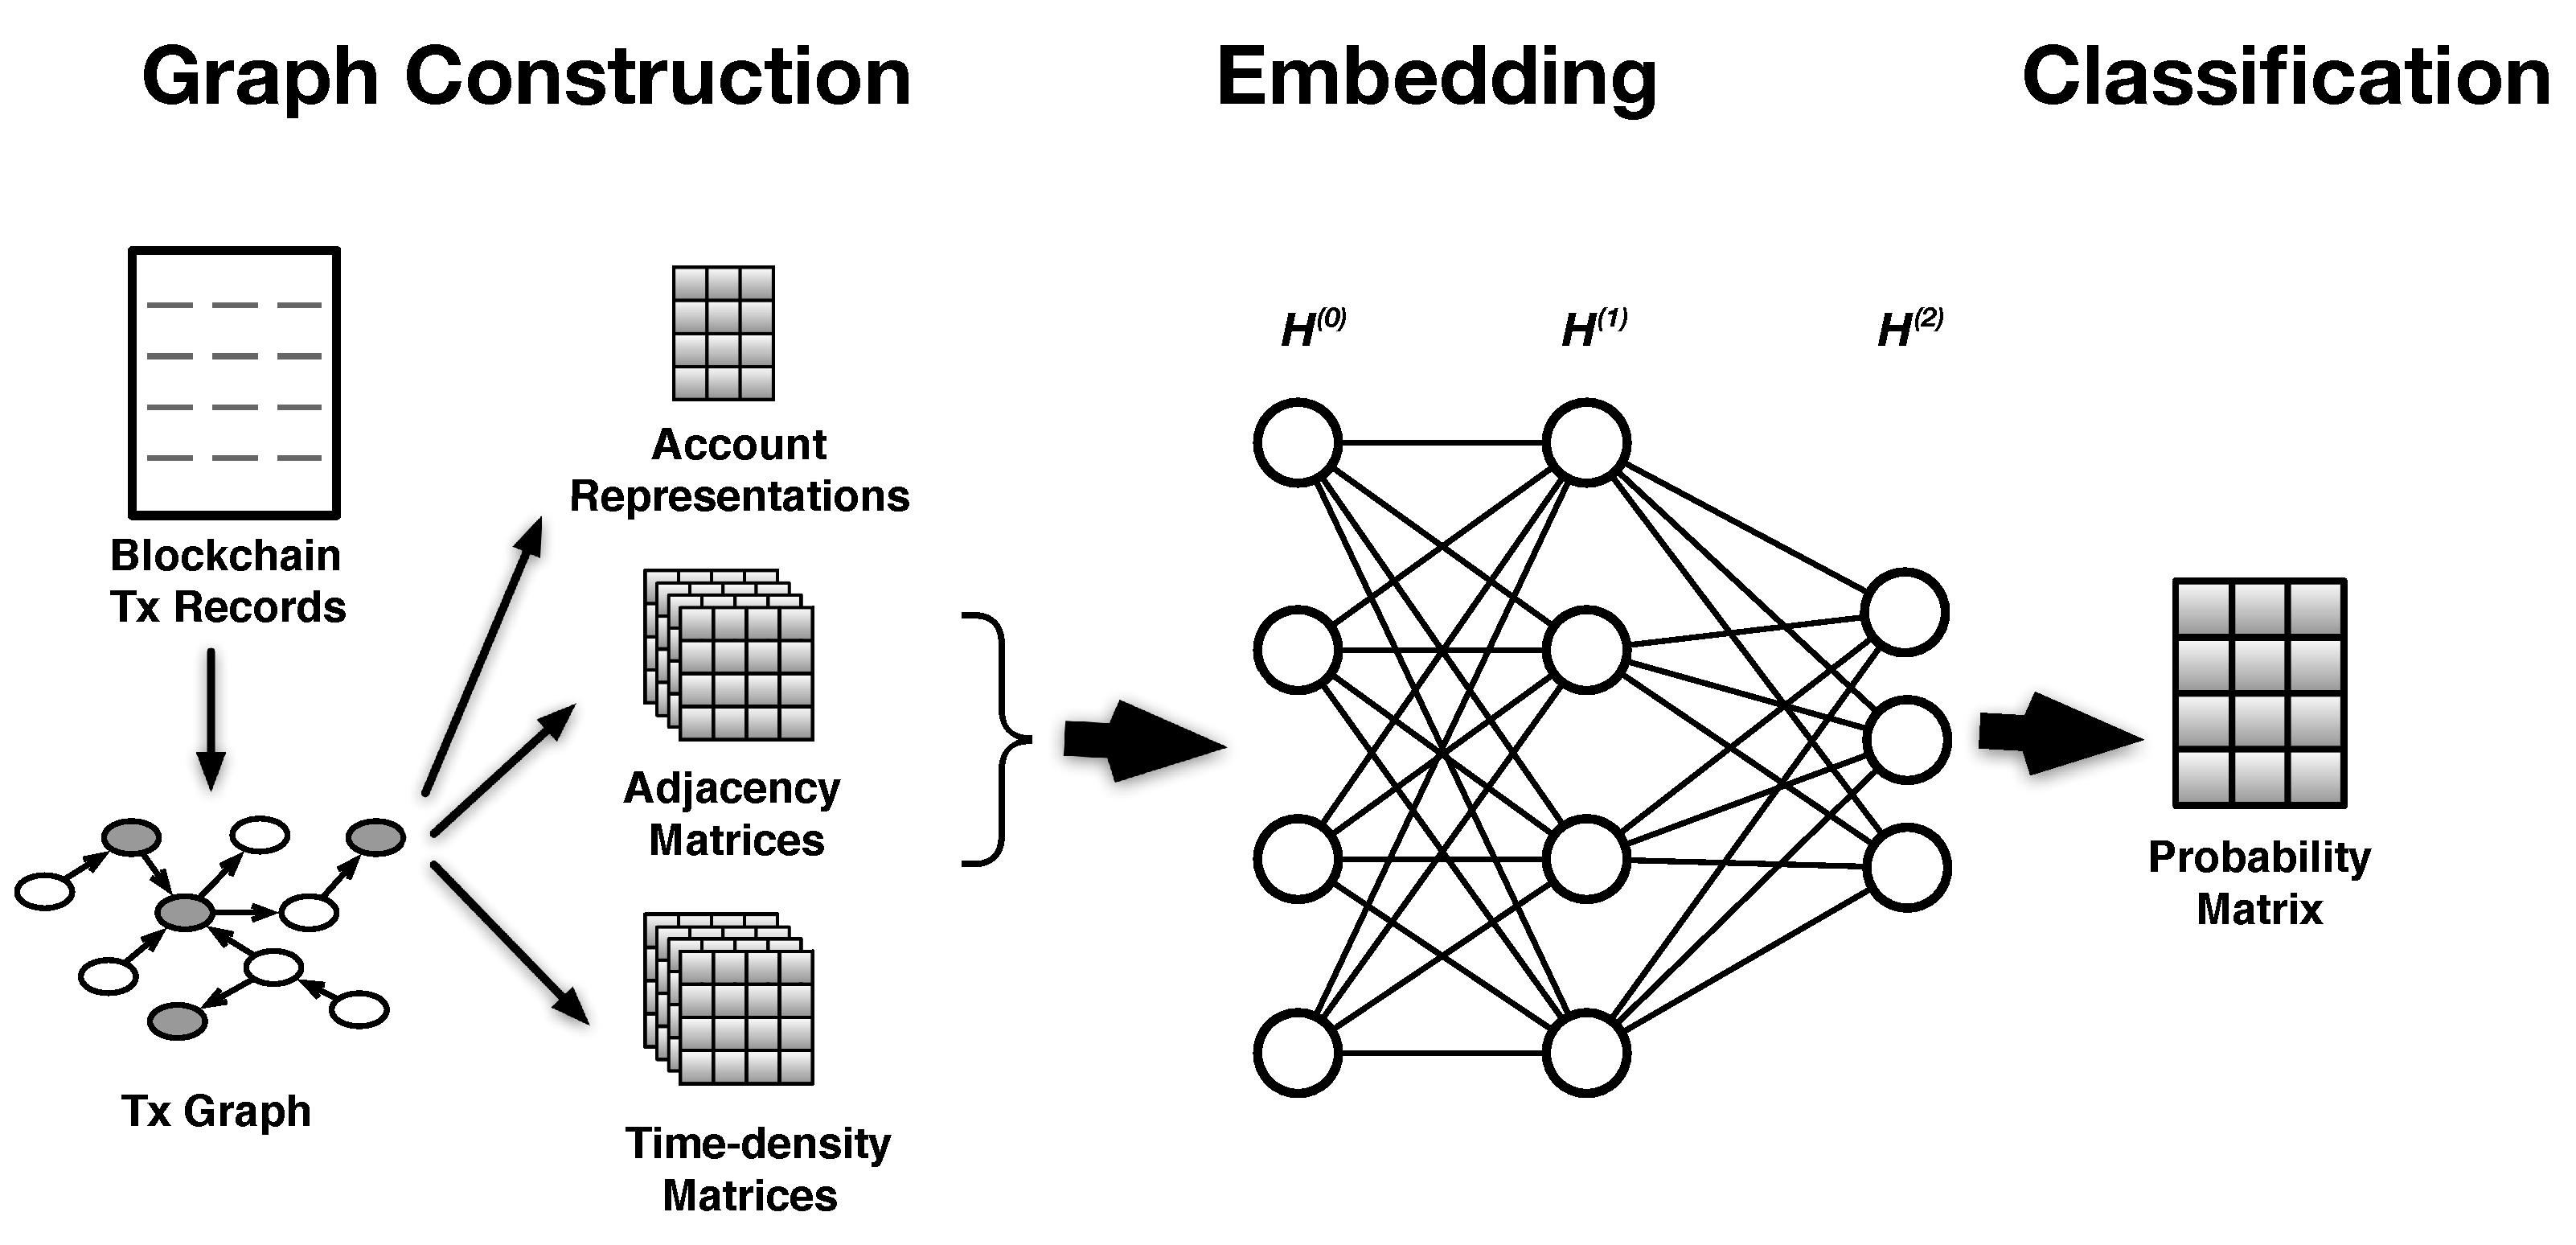
\includegraphics[width=3.5in]{fig/architecture.eps}
	\caption{Overall architecture.}
	\label{fig:architecture}
\end{figure}

\textbf{Phase 1: Graph construction}. We construct the blockchain transaction graph as a directed graph $G_{t}=(V,E)$, where node $v \in V$ represents an account which can be EOA and CA both. We use the terms account and node interchangeably in the remainder of this paper. And number of accounts is depicted as $|V|=N$.

$E$ is a set of ordered pairs, where $E=\{(v_i,v_j)|v_i,v_j \in V\}$. The order of an edge indicates the direction of transaction (e.g., assets transfer or smart contract invocation) from $v_i$ to $v_j$.%Analogously, the number of edges in ETG is represented as $|E|$.

\textbf{Phase 2: Graph embedding}.
The embedding process can be defined as follows: given $G_{t}=(V,E)$, we represent each node $v$ in a low-dimensional vector space $\vec{y_v}$, so that graph analysis algorithms can then be computed efficiently.

Typical network embedding techniques, such as random-walk based and deep learning based models, use the pure network structure to map into the embedding space~\cite{goyal2018capturing}. Our model is primarily motivated as an extension of GCNs (Graph Convolutional Networks)~\cite{kipf2016semi,schlichtkrull2018modeling}, which puts the features of nodes and edges into the representation, since it shows effectiveness for entity classification in large-scale relational data.


\textbf{Phase 3: Node classification}.
The final objective of our approach is to predict account identities on transaction graph. By given a labeled accounts set, supervised or semi-supervised methods can be used for entities classification. A intuitive way is simply stacking GCN layers of the form with a softmax ($\cdot$) activation on the output of the last layer~\cite{schlichtkrull2018modeling}. A cross-function can be the minimizing objective for training.

The categorization is important to performance of classification as well. To be frank, the perfect categorization does not exist because Ethereum and Ethereum-like blockchains are still in a development stage. \textcolor{red}{For accounts in Ethereum, we propose} a coarse but effective taxonomy.



\subsection{Graph Construction}
The transaction graph can be constructed based on original transaction records synchronized from the blockchain. In AIGL, the graph is represented as several matrices: (a) \emph{account representations}, (b) \emph{adjacency matrices}, and (c) \emph{time density matrices}.


%(1) a node representation matrix that captures the structural and additional information of accounts, (2) a list of adjacency matrices which describe different relations, and (3) a list of time-density matrices that represent transaction intensiveness between each pair of nodes.

%Different from other studies~\cite{kipf2016semi,schlichtkrull2018modeling}, the graph is translated into 

\paragraph{Account representations} To encode the overall structural and additional information of accounts, we \textcolor{red}{denote the account representations as} a feature matrix $X \in \mathbb{R}^{N \times d}$. In matrix $X$, each account contains the following $d$ pre-defined features.

\begin{itemize}
	\item \emph{in-degree}: the number of incoming edges of a node, that is, the number of transactions initiated by an account.
	\item \emph{out-degree}: the number of outgoing edges of a node, that is, the number of transactions which point to an account.
	\item \emph{weighted in-degree}: the value summation of incoming edges of a node, which represents the total crptocurrencies received by an account.
	\item \emph{weighted out-degree}: the value summation of edges outgoing to a node, which represents the total cryptocurrencies sent from an account.
	%\item eccentricity
	%\item clustering coefficient
	\item \emph{account type}: whether the account is a smart contract or normal one.
\end{itemize}

\paragraph{Multi-relations} Different from other networks, edges in transaction graph stand for heterogeneous activities such as money transfer, contract creation and contract invocation. \textcolor{red}{Obviously, such} multi-relations can not be measured in a uniform weighted model.

To address the challenge, we divide the raw transaction graph into several sub-graphs and capture the relations of graph neighboring nodes using adjacent matrices. The set of adjacency matrices, $\{A^1,A^2,\dots,A^R|A^i\in \mathbb{R}^{N \times N}\}$, describes the $R$ relations among $N$ nodes in transaction graph. It is conceivable that, the strategy of division has a large influence on classification performance.

\textcolor{red}{In AIGL, four major transactions are considered,} including \texttt{CALL} with value, \texttt{CALL} without value, \texttt{CREATION} and \texttt{REWARD}, which represent the relations of cryptocurrency transferring, smart contract invocation, smart contract deployment and mining rewarding, respectively. 

\textcolor{red}{On one hand,} for relations of \texttt{CALL} without value, \texttt{CREATION} and \texttt{REWARD}, we calculate the frequency of repeated edges between a pair of nodes as the adjacent weight in the corresponding relation adjacent matrix. For cryptocurrency transferring, on the other hand, it is not sensible to use the assets amount directly as the adjacent weight. That is because the accounts have varied enormously in terms of cryptocurrency transferring which will lead to underflow and overflow in the process of training.

 Taking Ethereum transaction as an example, the amount of assets transferring is discretized into three ranges: (1) small transfers which the transaction value is less than 1 ETH (the cryptocurrency used in Ethereum); (2) medium transfers which the transaction value is between 1 ETH and 10 ETH and (3) major transfers which the transaction value is above 10 ETH. Then the ETH transferring matrix can be calculated in a similar way with other relations.

%forward transactions introduced above and 4 reverse relations in order to pass information from the opposite direction. Besides, a self loop as a special relation type is included to retain information of the previous layer in the GCN network.

%Specially, the adjacent matrices are modified to preserve the asymmetric proximity of transaction graph, which will be addressed in detail later.

\paragraph{Time-density matrices}
Even in a single relation graph, there may be multiple edges between the same node pairs. This occurs quite naturally since an account may transfer or invoke to another account repeatedly for a period of time which is quite different from the knowledge graphs and citation networks.

Intuitively, a simple solution is to merge those edges by frequency or weight summation \textcolor{red}{in the same way as what is doing in adjacency matrices. In fact, each transaction is labeled with block height which can be considered timestamp these repeated edges are located at different time intervals along the time axis}. 
 
\begin{figure}[htbp]
\centering
\begin{tabular}{c}
	\subfigure[Time variance histogram of whole nodes.]{
		\label{fig:high_order}
		%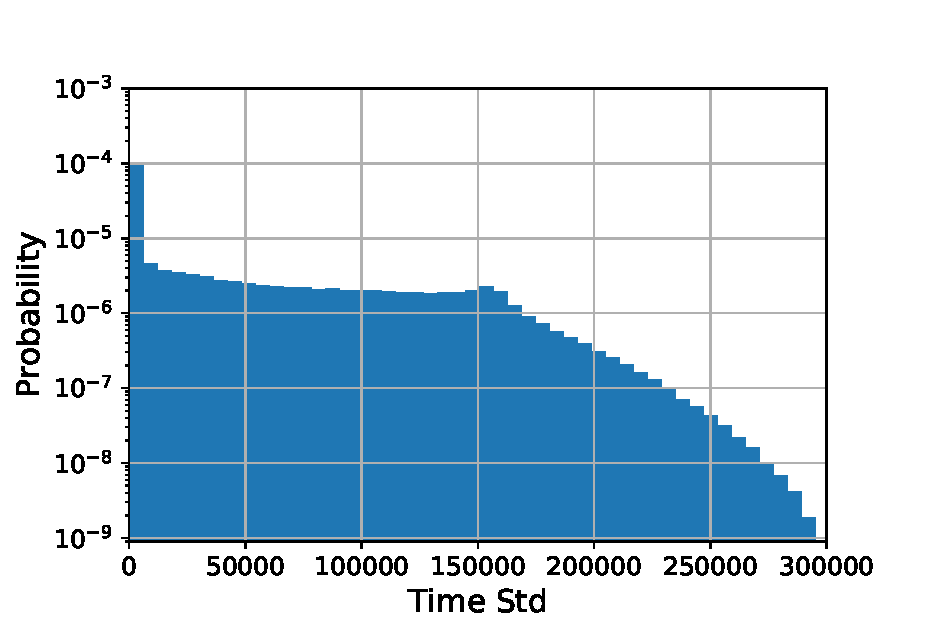
\includegraphics[width=0.22\textwidth]{fig/all_time_std_pdf.eps}
    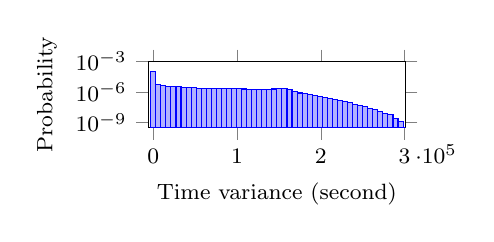
\begin{tikzpicture}
\begin{axis}[ymax=0.001,ybar,ymode=log,bar width=6023.807139652907,log origin=infty,xmin=-6023.807139652907,ytick align=outside,enlargelimits=0,
width=.40\textwidth,
height=.20\textwidth,
ylabel=Probability,
xlabel=Time variance (second),
every x tick scale label/.style={at={(xticklabel cs:1)},anchor=south west},
  label style={font=\footnotesize},
tick label style={font=\footnotesize} ,
]
\addplot  plot coordinates {
(0.0, 9.451382865223466e-05)
(6023.807139652907, 5.4237855234498505e-06)
(12047.614279305813, 4.160561994558263e-06)
(18071.421418958722, 3.567714777734051e-06)
(24095.228558611627, 3.385128656276782e-06)
(30119.03569826453, 3.165308635083816e-06)
(36142.842837917444, 2.9615307529739165e-06)
(42166.64997757035, 2.6626153921894407e-06)
(48190.45711722325, 2.5490152149843527e-06)
(54214.26425687616, 2.3890921746281617e-06)
(60238.07139652906, 2.275444535473124e-06)
(66261.87853618198, 2.248248838151831e-06)
(72285.68567583489, 2.156718467673447e-06)
(78309.49281548779, 2.138350693042835e-06)
(84333.2999551407, 2.0591366985764506e-06)
(90357.1070947936, 2.0862137410228693e-06)
(96380.9142344465, 2.0135969575995206e-06)
(102404.72137409942, 2.000948347937872e-06)
(108428.52851375232, 1.9544830989369192e-06)
(114452.33565340523, 1.9188391745245435e-06)
(120476.14279305813, 1.8834088288869425e-06)
(126499.94993271104, 1.8642104701322076e-06)
(132523.75707236395, 1.8633324240581345e-06)
(138547.56421201685, 1.8347365992133192e-06)
(144571.37135166978, 1.9392715439779758e-06)
(150595.17849132267, 2.1352419353211166e-06)
(156618.98563097557, 2.1487685910568386e-06)
(162642.79277062847, 1.6649889352174985e-06)
(168666.5999102814, 1.0367825656806102e-06)
(174690.4070499343, 7.939434987619423e-07)
(180714.2141895872, 6.496829018892185e-07)
(186738.02132924012, 5.151757357311993e-07)
(192761.828468893, 4.3131047016972446e-07)
(198785.6356085459, 3.5105231280444205e-07)
(204809.44274819884, 2.852225882239295e-07)
(210833.24988785174, 2.272003544101756e-07)
(216857.05702750463, 1.7961974958539996e-07)
(222880.86416715756, 1.4827113164349042e-07)
(228904.67130681046, 1.1445449230418602e-07)
(234928.47844646336, 8.545524088479658e-08)
(240952.28558611625, 6.371766780774196e-08)
(246976.09272576918, 4.777045262457526e-08)
(252999.89986542208, 3.780344313509607e-08)
(259023.70700507498, 2.6009148572545693e-08)
(265047.5141447279, 1.8557622430411254e-08)
(271071.3212843808, 1.31232291611476e-08)
(277095.1284240337, 8.305841241232658e-09)
(283118.9355636866, 5.624241069063257e-09)
(289142.74270333955, 2.7053311471443514e-09)
(295166.54984299245, 1.3526655735721757e-09)
(301190.35698264535, 3.0850267467435584e-10)
};\end{axis}
\end{tikzpicture}

	%\caption{Example of a high-order proximity caption.}
	}\\
	\subfigure[Time variance histogram of hack\&phish nodes.]{
		\label{fig:asymmetric}
		%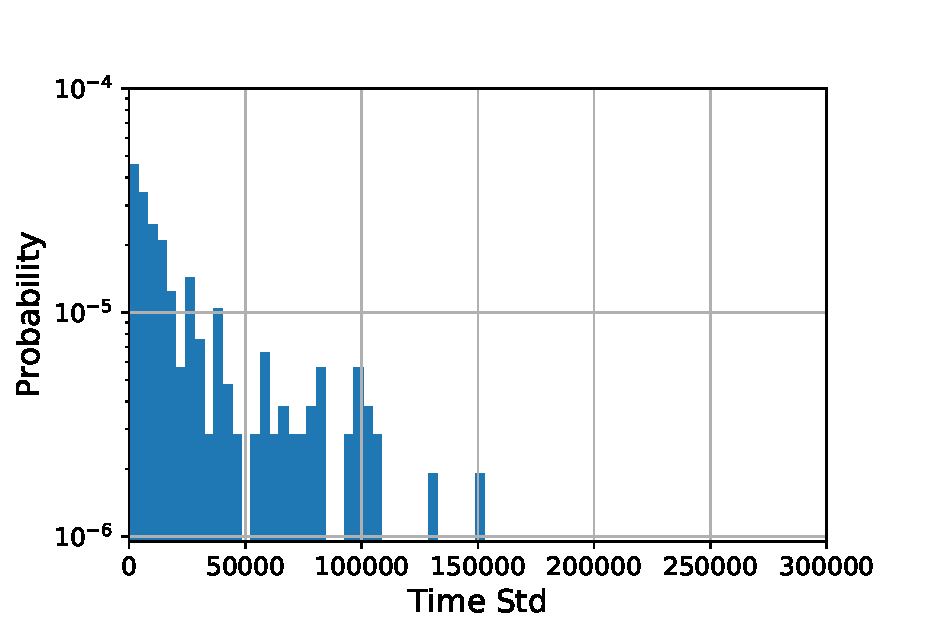
\includegraphics[width=0.22\textwidth]{fig/fake_time_std_pdf.eps}
    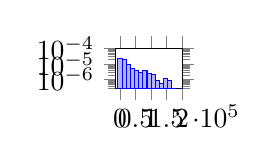
\begin{tikzpicture}
\begin{axis}[ymax=0.0001,ybar,ymode=log,bar width=13410.783587930588,log origin=infty,xmin=-13410.783587930588,ytick align=outside,enlargelimits=0,
width=.20\textwidth,
every x tick scale label/.style={at={(xticklabel cs:1)},anchor=south west},
]
\addplot  plot coordinates {
(0.0, 2.1630081044550223e-05)
(13410.783587930588, 1.9637836737815332e-05)
(26821.567175861175, 8.822796215540222e-06)
(40232.350763791765, 5.122913931604e-06)
(53643.13435172235, 3.699882283936222e-06)
(67053.91793965294, 2.8460632953355556e-06)
(80464.70152758353, 3.984488613469778e-06)
(93875.48511551411, 2.561456965802e-06)
(107286.2687034447, 2.2768506362684445e-06)
(120697.0522913753, 8.538189886006666e-07)
(134107.83587930587, 5.692126590671111e-07)
(147518.61946723645, 1.1384253181342222e-06)
(160929.40305516706, 8.538189886006666e-07)
(174340.18664309764, 2.8460632953355556e-07)
(187750.97023102822, 0.0)
(201161.75381895882, 2.8460632953355556e-07)
};\end{axis}
\end{tikzpicture}

	}
\end{tabular}
\caption{Examples.}
\label{fig:time_std}
\end{figure}

Fig.~\ref{fig:time_std} illustrates the distribution of time variance when transaction happens of whole accounts and hack \& phish accounts in Ethereum. It is not difficult to find that the time variance distribution of hack \& phish accounts is more concentrated compared with other accounts, which seems perfectly reasonable since the hacks and phishes are more active in a short time. This insight inspires us to use time information such as the variance of time transaction happens.

To describe time-density information, we use a set of matrices $\{K^1,K^2,\dots,K^R|K^i\in \mathbb{R}^{N \times N}\}$. Given a sequence $\{h_{ij1}^r,h_{ij2}^r,\dots,h_{ijm}^r | h_{ijk}^r>0\}$ as the block height of transactions in relation $r$ between node $v_i$ and $v_j$, the time-density of each relation $r$ is computed as%Equation \ref{eq:time}

\begin{equation}
k_{ij}^r=g(\sqrt{Var[\frac{1}{m}\sum_{k=1}^m h_{ijk}^r]})
\label{eq:time}
\end{equation}

\noindent where $g(\cdot)$ is the function of squash which can be logarithmic function.

\subsection{Embedding}
\label{sec:rGCN layers}
Based on the above input matrices, we propose a multi-layer Graph Convolutional Network with the following layer-wise propagation rule:

%The method can be understood as a more abstract propagation rule:
\begin{equation}
H^{(l+1)}=\delta(\sum_{r\in R} (K^r\odot (D^r)^{-1}A^r)H^{(l)}W_r^{(l)})
\end{equation}
\noindent where $H^{(l)}$ is the matrix of activations of the $l$-th layer, and here the $0$ layer is set as the account representations, that is, $H^{(0)}=X$. We use $\delta(\cdot)$ to denote an activation function such as the ReLU$(\cdot)$ = max$(0,\cdot)$, $D^r$ is a diagonal matrix where $D^r_{ii}=\sum_{j}A^r_{ij}$, and $A^r$ is the adjacent matrix of relation $r$. $\odot$ indicates point-wise multiplication.

The edge weight $A_{ij}$ in adjacency matrix $A$ is defined as \emph{first-order proximity} which represents similarity between nodes $v_i$ and $v_j$~\cite{tang2015line}. Further, \emph{second-order proximity} compares the neighborhood of two nodes and treat them as similar if they have a similar neighborhood~\cite{goyal2018graph}.

In cryptocurrency transaction graph, \textcolor{red}{it turns out that second-order proximity plays important role}  in preserving the local structure as well as first-order proximity. As shown in Figure \ref{fig:high_order}, nodes $a$ and $c$ are smart contracts and node $b$ is normal user. Obviously, $a$ is not adjacent to $c$  but they have similar neighbor structure. Embedding models with first-order proximity will keep them far apart although they have similar connection structures, while embedding with second-order proximity captures this similarity.

 We feed the input into a \textcolor{red}{GCN} model with 2 hidden layers, as a trade-off between preserving second-order proximity and introducing noise. 
 
 The input of the $l$-th layer is $H^{(l)}=\{h_1^{(l)},h_2^{(l)},...,h_N^{(l)}|h_i^{(l)}\in \mathbb{R}^{N \times d^{(l)}}\}$. Hence the method can be understood as special cases of the forward updating process.

\begin{equation}
h_i^{(l+1)}=\delta(\sum_{r\in R} \sum_{j \in N_i^r} \frac{\tau_{ij}^r}{\hat c_{i,r}}W_r^{(l)}h_j^{(l)})
\end{equation}

\noindent where $h_i^{(l)}$ is the hidden state of node $v_i$ in the $l$-th layer of the neural network. $r \in R$ represents a kind of relation, $N_i^r$ denotes the set of neighbor indices of node $v_i$ under relation $r$, and $k_{ij}^r$ is the time-density of transactions from node $v_i$ to $v_j$ which is represented in Eq.~(\ref{eq:time}).



\begin{figure}[htbp]
	\centering
	\subfigure[Second-order proximity]{
		\label{fig:high_order}
    \begin{tikzpicture}
\tikzset{
  base/.style={draw, on grid, align=center, minimum height=2.8ex},
  pn/.style={base, circle},
}


\tikzmath{\r=1.2;}

\node [pn, thick] (a) at (0, 0) {};
\node at (a) {\footnotesize a};
\node [pn, thick] (b) at (\r, 0) {};
\node at (b) {\footnotesize b};
\node [pn, thick] (c) at (2*\r, 0) {};
\node at (c) {\footnotesize c};

\node[pn, thick] (a1) at ({\r*cos(60)}, {\r*sin(60)}) {};
\node[pn, thick] (a2) at ({\r*cos(120)}, {\r*sin(120)}) {};
\node[pn, thick] (a3) at ({\r*cos(180)}, {\r*sin(180)}) {};
\node[pn, thick] (a4) at ({\r*cos(240)}, {\r*sin(240)}) {};
\node[pn, thick] (a5) at ({\r*cos(300)}, {\r*sin(300)}) {};

\node[pn, thick] (b1) at ({2*\r + \r*cos(60)}, {\r*sin(60)}) {};
\node[pn, thick] (b2) at ({2*\r + \r*cos(120)}, {\r*sin(120)}) {};
\node[pn, thick] (b3) at ({2*\r + \r*cos(0)}, {\r*sin(0)}) {};
\node[pn, thick] (b4) at ({2*\r + \r*cos(240)}, {\r*sin(240)}) {};
\node[pn, thick] (b5) at ({2*\r + \r*cos(300)}, {\r*sin(300)}) {};

\draw[->, >=stealth, thick] (a1)-- (a);
\draw[->, >=stealth, thick] (a2) -- (a);
\draw[->, >=stealth, thick] (a3) -- (a);
\draw[->, >=stealth, thick] (a4) -- (a);
\draw[->, >=stealth, thick] (a5) -- (a);

\draw[->, >=stealth, thick] (b1) -- (c);
\draw[->, >=stealth, thick] (b2) -- (c);
\draw[->, >=stealth, thick] (b3) -- (c);
\draw[->, >=stealth, thick] (b4) -- (c);
\draw[->, >=stealth, thick] (b5) -- (c);

\draw[->, >=stealth, thick] (b) -- (a) node [midway, above] {\scriptsize invoke};
\draw[->, >=stealth, thick] (b) -- (c) node [midway, above] {\scriptsize invoke};
\end{tikzpicture}

		%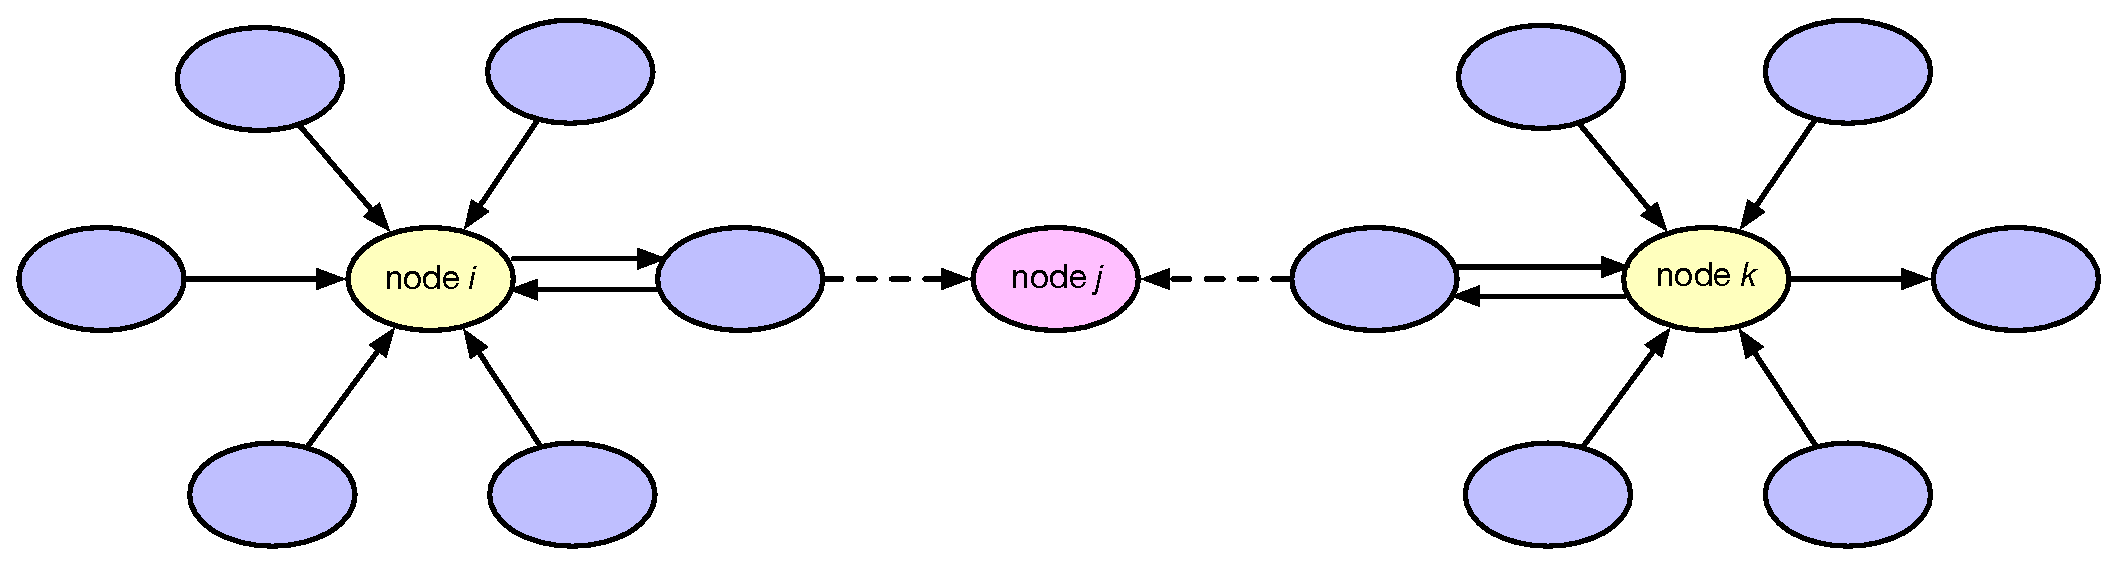
\includegraphics[width=2.0in]{fig/high_order_proximity.eps}
	%\caption{Example of a high-order proximity caption.}
	}
	\subfigure[Asymmetric proximity]{
		\label{fig:asymmetric}
    \begin{tikzpicture}
\tikzset{
  base/.style={draw, on grid, align=center, minimum height=2.8ex},
  pn/.style={base, circle},
}


\tikzmath{\r=1.2;}

\node [pn, thick] (a) at (0, 0) {};
\node at (a) {\footnotesize a};
\node [pn, thick] (b) at (\r, 0) {};
\node at (b) {\footnotesize b};
\node [pn, thick] (c) at (2*\r, 0) {};
\node at (c) {\footnotesize c};

%\node[pn] (a1) at ({\r*cos(60)}, {\r*sin(60)}) {};
%\node[pn] (a2) at ({\r*cos(120)}, {\r*sin(120)}) {};
%\node[pn] (a3) at ({\r*cos(180)}, {\r*sin(180)}) {};
%\node[pn] (a4) at ({\r*cos(240)}, {\r*sin(240)}) {};
%\node[pn] (a5) at ({\r*cos(300)}, {\r*sin(300)}) {};

\node[pn, thick] (b1) at ({2*\r + \r*cos(360.0/14)}, {\r*sin(360.0/14)}) {};
\node[pn, thick] (b2) at ({2*\r + \r*cos(360.0*3/14)}, {\r*sin(360.0*3/14)}) {};
\node[pn, thick] (b3) at ({2*\r + \r*cos(360.0*5/14)}, {\r*sin(360.0*5/14)}) {};
\node[pn, thick] (b4) at ({2*\r + \r*cos(360.0*9/14)}, {\r*sin(360.0*9/14)}) {};
\node[pn, thick] (b5) at ({2*\r + \r*cos(360.0*11/14)}, {\r*sin(360.0*11/14)}) {};
\node[pn, thick] (b6) at ({2*\r + \r*cos(360.0*13/14)}, {\r*sin(360.0*13/14)}) {};

%\draw[->, >=stealth] (a1)-- (a);
%\draw[->, >=stealth] (a2) -- (a);
%\draw[->, >=stealth] (a3) -- (a);
%\draw[->, >=stealth] (a4) -- (a);
%\draw[->, >=stealth] (a5) -- (a);

\draw[->, >=stealth, thick] (b1) -- (c);
\draw[->, >=stealth, thick] (c) -- (b2);
\draw[->, >=stealth, thick] (b3) -- (c);
\draw[->, >=stealth, thick] (c) -- (b4);
\draw[->, >=stealth, thick] (b5) -- (c);
\draw[->, >=stealth, thick] (c) -- (b6);

\draw[->, >=stealth, thick] (a) -- (b) node [midway, above] {\scriptsize deposit};
\draw[->, >=stealth, thick] (b) -- (c) node  {};
\draw[->, >=stealth, thick] (c) to [out=205, in=335]  node [midway, below] {\scriptsize
withdrawal}  (a);
\end{tikzpicture}

		%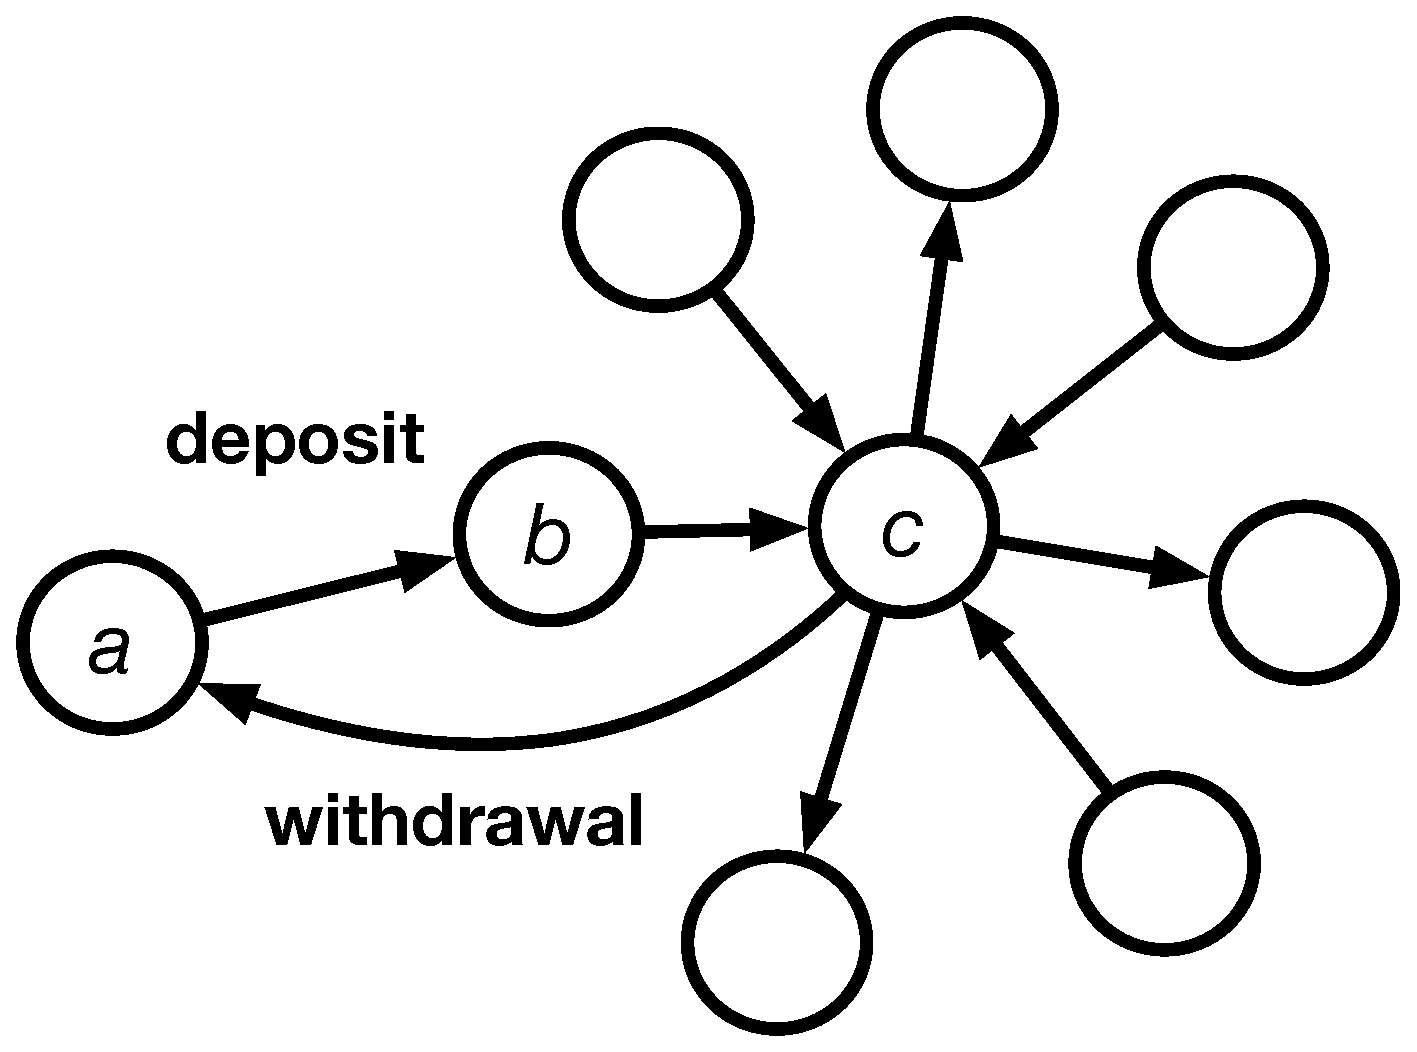
\includegraphics[width=1.5in]{fig/asymmetric.eps}
	}
	\caption{Examples of second-order and asymmetric proximity.}

\end{figure}


\textcolor{red}{Another overlooked closeness, \emph{asymmetric proximity}} should also be preserved in transaction graph. For instance, as shown in Figure. \ref{fig:asymmetric}, \textcolor{red}{node $a$ denotes cryptocurrency trader and node $b$ and $c$ are cryptocurrency exchange accounts. Consequently, edge $(a,b)$ stands for deposit process while edge $(c,a)$ is withdrawal process.} Generally, edge weight can be $A_{ab}=A_{bc}=A_{ca}$ since deposit and withdrawal come in pairs in symmetric model. However, the proximity $(a,c)$ is not equal to proximity $(c,a)$ due to their asymmetric local structures.

Unlike the asymmetric proximity preserving approach based on random walk~\cite{zhou2017scalable}, our method is based on a kind of non-probability graph embedding model.
 %Zhou et. proposed a scalable asymmetric proximity preserving graph embedding method based on random walk~\cite{zhou2017scalable}. In their model, the probability that $v_a$ arrives at $v_c$ is far less than the one that $v_c$ arrives at $v_a$, as the out degree of $v_c$ is bigger than the out degree of $v_a$
 
To preserve the asymmetric proximity, the coefficient $\hat c_{i,r}$ is introduced as:
\begin{equation}
\hat c_{i,r}=\frac{1}{d_i^r\cdot |N_i^r|}
\end{equation}

\noindent where $d_i^r=\sum_{j}A^r_{ij}$, and $|N_i^r|$ is used for normalization.



\subsection{Node Classification}
The output of the last layer indicates the probability that each node being assigned to each class.

The output of the last \textcolor{red}{GCN} layer is regarded as a probability matrix $P=\{p_1,p_2,...,p_N|p_i\in \mathbb{R}^{N \times m}\}$, where $p_i=\{p_{i,1},p_{i,2},...,p_{i,m}\}$ describes the probability of classifying node $v_i$ into $m$ categories.

We utilize the cross-entropy loss function as the training objective:
\begin{equation}
L=-\sum_{i=1}^T\sum_{j=1}^m y_{i,j}\log p_{i,j}+\lambda ||\theta||^2
\end{equation}

\noindent where $T$ is the number of training samples, $y_{i,j}$ is the true probability of node $v_i$ belonging to category $j$. $\theta$ is the set of all parameters and $\lambda$ is the coefficient for $L_2$  regularization.
